\documentclass{article}
\usepackage[utf8]{inputenc}
\usepackage{xurl}
\usepackage{graphicx}
\usepackage[style=chem-acs, articletitle=true]{biblatex}
\addbibresource{references.bib}
\graphicspath{ {./images/} }
\usepackage[table]{xcolor}
\setlength{\arrayrulewidth}{0.1mm}
\setlength{\tabcolsep}{18pt}
\renewcommand{\arraystretch}{1.3}
\arrayrulecolor[HTML]{000}
\begin{figure}[ht!]
    \begin{center}
    
\includegraphics[height=1.7cm]{CU.jpg}
    \end{center}
\title{SOEN 6461  PROJECT\\Deliverable 1}
\author{DEPARTMENT OF COMPUTER SCIENCE\\AND SOFTWARE ENGINEERING\\\\
SOEN 6461: SOFTWARE DESIGN\\METHODOLOGIES\\\\
WINTER 2023\\\\
\textbf{Submitted to:} \textit{Dr. Pankaj Kamthan}\\\\
\textBf{By,}
\textbf{Team E}\\\\
\textit{Nithin Reddy Indurthi (ID: 40181743)}\\
\textit{Mayurkumar Kanubhai Jodhani (ID: 40230634)}\\
\textit{Venkat Sai Janumpally (ID: 40201444)}\\
\textit{Nithin Harikrishnan (ID: 40227651)}\\
\textit{Abhishek Gupta (ID: 40226797)}}

\date{March 6, 2023}
\usepackage{hyperref}
This report aims to create a set of interrelated artifacts for the problem as well as the solution domain, involving elements of
both agile methodologies and rigid methodologies. The work on iGo has been divided into a five interrelated problems to be
solved as a team and individually. 
\usepackage{graphicx}
\begin{document}

\maketitle
\end{figure}

\graphicspath{ {./images/}

\newpage
\tableofcontents
\listoffigures
\newpage
\section{Introduction}
\textbf  
A ticket machine, also referred to as a ticket vending machine (TVM)\cite{VERBICH201743}, is an automated device that dispenses paper or electronic tickets, or reloads a stored-value or smart card, or a mobile wallet on the user's smartphone. These machines are commonly found at railway stations, metro stations, and some tram stops and trams, where they dispense train tickets, transit tickets, and tram tickets, respectively.
\\\
\\\
A vending machine is a machine that dispenses goods or services in exchange for money or electronic payments. With the advantage of low hardware cost and the high cost of human labor, vending machines nowadays offer a wide range of products and services. Transport Ticket Vending Machines (TVMs) belong to a major category of vending machines, which primarily facilitate the recharge of transit fares through smart cards and dispense paper tickets or transit passes based on the user's input, such as the type and quantity of the tickets, and appropriate payments\cite{siebenhandl2013user}. 
\\\
\\\
Furthermore, TVMs are used to help manage queues and prioritize services. For our project, we have selected the TVMs used by Société de transport de Montréal (STM), which are widely distributed in all metro stations across the greater Montreal area. We chose this specific TVM because its user interface and functionality are familiar to the project team members.
\section{Problem 1: Chosen TVM}
Our project focuses on the TVM system used in the Montreal STM metro network, which comprises a total of 68 metro stations covering an operational network length of 69.2km. This operational network is categorized into four different lines, namely Green, Orange, Yellow, and Blue. The Orange line is the longest, spanning 30km and featuring 31 metro stops or stations, running from Cote-Vertu to Montmorency.
\\\
\\\
To enable the public to purchase tickets or recharge their smart cards (OPUS cards), one or two TVMs (Ticket Vending Machines) are typically installed in each station. 
The chosen TVM has the following characteristics:
 \textbf{\subsection{UI functionality:}}
The TVM's user interface is designed to be intuitive, requiring little to no training for users to understand its functionality. Moreover, the interface assumes minimal prior knowledge or skill level from its users. The interface is constructed to reduce cognitive interference caused by stress and to support user tasks, minimizing the possibility of errors. The user interface features physical buttons for selecting user choices, a physical keyboard, and a simple color display\cite{jiang2013simulation}.
\\\
\\\
Taking inspiration from the existing design, we suggest incorporating a touch-sensitive color display in our proposed design. Touch-sensitive displays are useful in building tangible user interfaces that can be customized based on user needs. 
\\\
\\\
Our design will also cater to the requirements of seniors and users with physical and cognitive constraints, such as those with limited vision or difficulties with physical movement. For instance, the keypad will be set at a height of 50cm, with an almost diagonal inclination angle (45 degrees) to facilitate wheelchair users. In addition, we will use tactile marking and indented keypads to provide assistance for visually impaired users, with voice assistance also available.
\textbf{\subsection{Payment methods:}}
The TVM system displays prices exclusively in Canadian dollars (CAD) and accepts CAD bills in denominations of five, ten, and twenty dollars, as well as coins worth one and two dollars and twenty-five cents. Users also have the option to pay with credit or debit cards. The TVM's outer body is constructed using sturdy materials to deter theft and vandalism, and the system includes built-in network security components to prevent fraudulent usage and ensure secure transactions with the bank.
\textbf{\subsection{Type and mode of tickets:}}
The chosen TVM can issue transit passes and recharge transit smart cards for users. The passes available for purchase may vary in time range, such as daily, weekly, and monthly, or on a per-usage basis, such as five or ten passes. The TVM user interface also includes multilingual support, specifically for English and French, to comply with legal requirements for operation in Canada.
\textbf{\subsection{Receipts and Location:}}
The TVM system includes an option to receive an email receipt in addition to a paper-based one.
Currently, the TVM is strategically positioned either in the center of the metro station or near ingress/egress points, with signs indicating its location for enhanced visibility. Our proposed TVMs will also be located near important bus stops.
\section{Problem 2: UML Class Diagram}
\begin{figure}[!ht]
    \begin{center}
        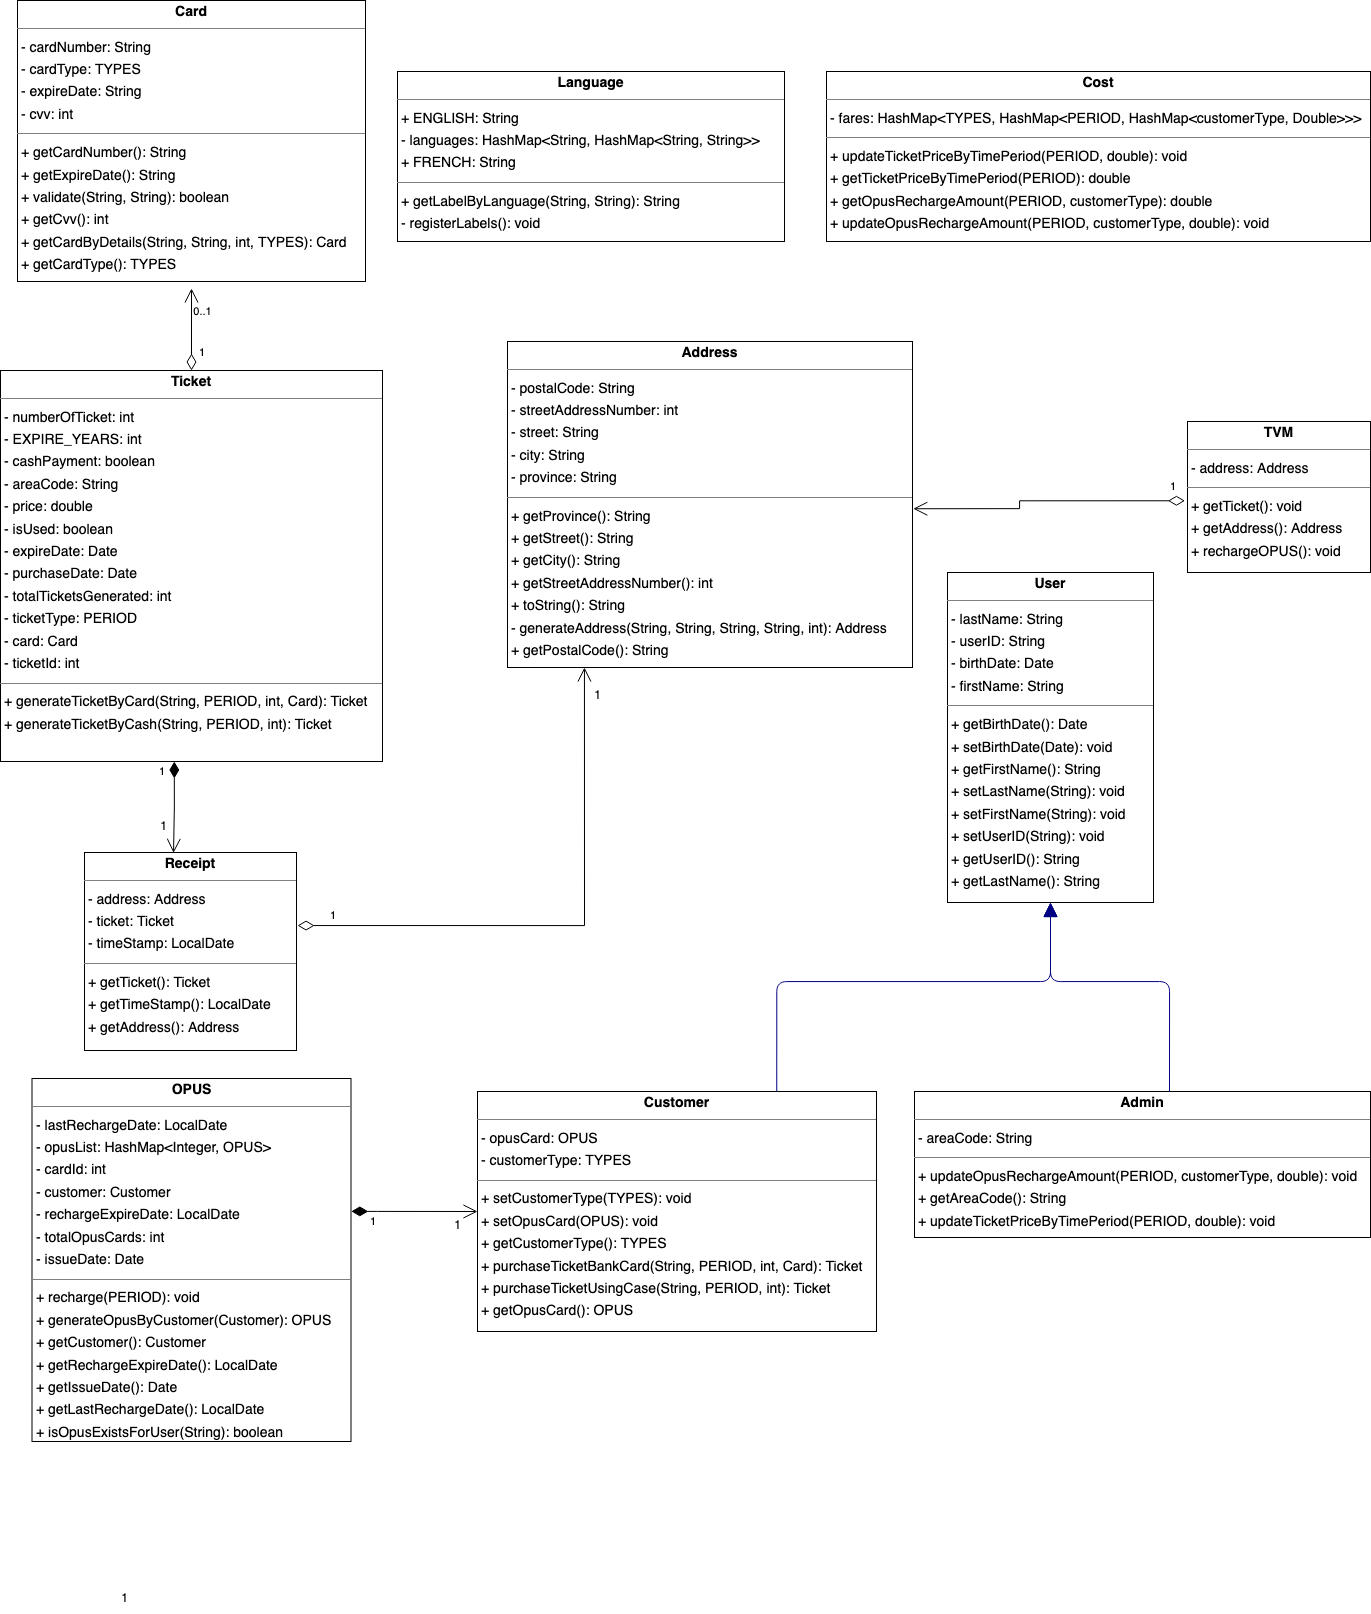
\includegraphics[width=4in]{class.png}
        \caption{Class Diagram}
    \end{center}
\end{figure}
\textbf{\subsection{Classes and Relationships}}
The system architecture being discussed here caters to two distinct user types, namely the system administrator and the customers who use the Metro to travel across various regions. While both user types share some common attributes, these attributes are described under the user class to ensure consistency and standardization. However, the administrator class has access to additional operations, such as the ability to update ticket prices and OPUS card recharge prices for different areas. This feature ensures that the system remains flexible and adaptable to changing circumstances, ultimately enhancing user experience.

\newline
On the other hand, the customer class has access to their own set of functions, including the ability to purchase tickets and issue OPUS cards, which can be used to buy tickets and facilitate travel. These functionalities are designed to streamline the process of travelling across various regions via the Metro, ultimately improving overall user satisfaction.
\newline
\\\
By using a shared user class, the system can maintain a clear and organized structure, which can be easily navigated by both system administrators and customers. Moreover, the system has been designed to ensure that it can accommodate different payment methods for tickets, including cash and credit/debit cards. In addition, ticket types such as single trip, round trip, etc. have also been incorporated into the system, ensuring that users have access to various options to suit their individual needs.
\newline
\\\
Furthermore, the system incorporates a cost class to manage the different prices of tickets and OPUS card recharges. This feature enables administrators to update prices as necessary, ensuring that the system remains current and relevant. Additionally, a language class has also been included in the system to provide access to the system in both English and French, thereby enhancing accessibility and inclusivity for a wider range of users. Overall, the system has been designed to provide an efficient and user-friendly experience for all users, while also being flexible and adaptable to meet changing user needs.
\newline
\\
The TVM class acts as the user's entry point in the system architecture being described, enabling users to buy tickets using cash or the OPUS card.
The system creates a corresponding receipt for the user's records once a ticket has been produced.
\newline
\\
In addition, the TVM class provides essential details about the region it is situated in.With the help of this feature, the system can give users access to tickets that are local to their area, guaranteeing that the ticket they buy is valid for use in the desired area.The system can effectively handle the distribution of tickets across various areas by incorporating this feature within the TVM class, which enhances the overall user experience. 
\newline
\\
Overall, the TVM class is a critical component of the system architecture, serving as the entry point for users and ensuring that the ticket purchase process is efficient and user-friendly. By incorporating vital information about the area in which the TVM is located, the system can provide users with access to tickets specific to their location, thereby enhancing overall user satisfaction. Additionally, the system's security features ensure that users' personal and financial information is protected, instilling trust and confidence in the system's functionality.
\section{Problem 3: Interviews}
In software engineering and human computer interaction, interviews are commonly employed to gather requirements, understand the software system users, and identify positive and negative user experiences. In preparation for our project, we conducted interviews with individuals to inform the development of software artifacts. To ensure a diverse sample, we selected interviewees who met the following criteria:
\begin{enumerate}
  \item Different age groups
  \item Different backgrounds and countries
  \begin{itemize}
  \item Technical Users.
  \item Non-Technical Users
\end{itemize}
\end{enumerate}
As the TVM system is a technical software, we believed it was suitable to conduct interviews with individuals possessing a technical background, particularly in software engineering and mechanical engineering. To ensure comprehensive coverage, we utilized the Hourglass model for our semi-structured interviews, consisting of both open-ended and close-ended questions. We employed a combination of audio and video recordings during our interviews. In preparation, we conducted a Pilot Interview to refine our question list for the actual interviews.
\newline
\newline
\textbf{Sample questions for Interview about TVM: (which we found the best and used for interview recording)}
\begin{enumerate}
\item Have you been using the Public Transport?
\item Which public transport you use the most?
\item Have you used the TVM at the metro stations?
\item How do you find the user interface of the TVM?
\item Don’t you have an issue with the language used in the TVM?
\item Are you satisfied with the locations of TVM?
\item Would you like it to be placed in the bus stops?
\item How often do you recharge the OPUS card?
\item Do you use the monthly card or the student card?
\item Any difficulties faced while recharging the OPUS card?
\item How do you find the waiting period for recharging the OPUS card?
\item Would you want a reminder to be sent to your email address for
recharging the OPUS card?
\item How do you find the TVM with the specially abled people? Is it friendly?
\item Any suggestions for improvement?
\end{enumerate}
\textbf{Conclusions derived}
\\\
Based on the responses we got for the questions we asked our interviewees
we concluded that:
\begin{enumerate}
\item It is recommended to install TVM machines at locations beyond just the metro stations, such as central areas of the city and crowded bus stops, to increase convenience for the public in recharging their metro cards and purchasing tickets. This way, people can easily access TVMs even when they are away from metro stations. Our project has taken this into consideration while deciding location for our TVMs.
\item According to feedback received during interviews, providing an email receipt option in addition to the traditional paper-based receipt would be beneficial for users. This is because some users have experienced issues with losing paper receipts, which can be problematic, especially for those seeking reimbursement from their employer. Therefore, incorporating the email receipt feature would be more convenient and preferred by users.
\item A larger proportion of interviewees expressed the view that having an online mechanism to recharge their cards would be more convenient. This would offer greater flexibility to recharge their card without requiring them to leave their location.
\end{enumerate}
\section{Problem 4: Usecase Diagram}
\begin{figure}[!p]
    \begin{center}
        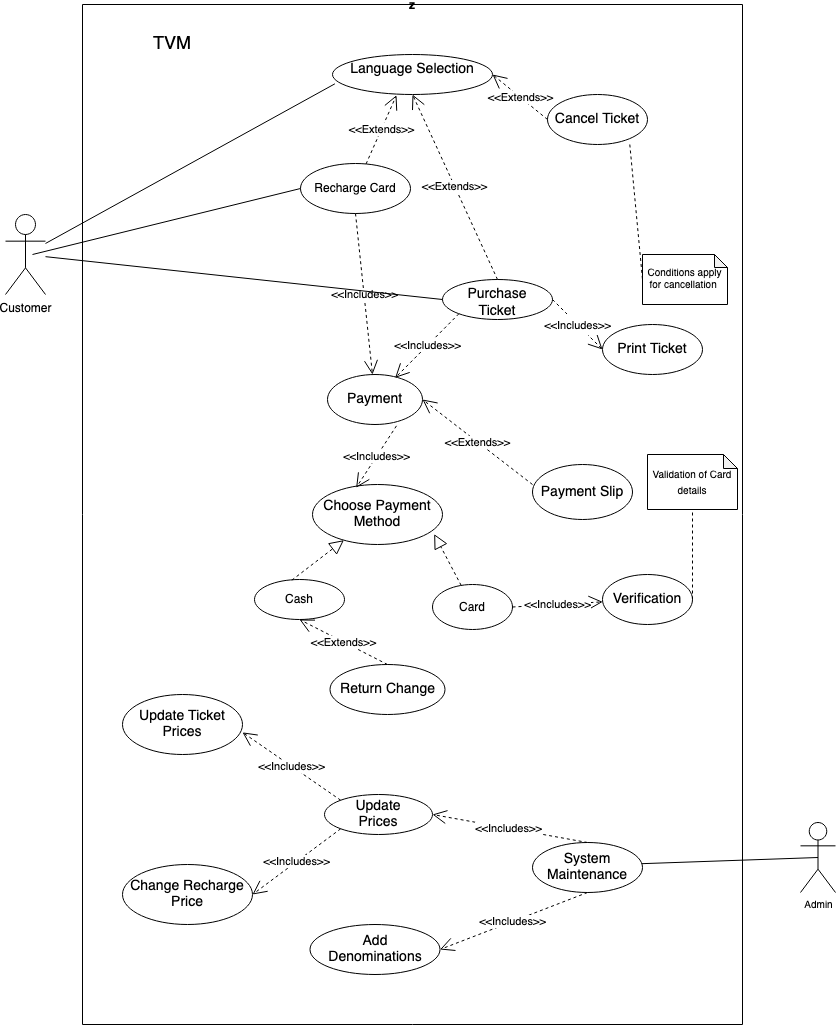
\includegraphics[width=5in]{UseCaseV2.drawio.png}
        \caption{Usecase Diagram}
    \end{center}
\end{figure}
\subsection{Language Selection}
\hskip1cm\
\begin{tabular}{|p{3cm}|p{6cm}|}
    \hline
    Name & Language Selection\\
    \hline
    Actors & Customer\\
    \hline
    Description & Customer selects one of two languages, French or English.\\
    \hline
    Trigger & A customer can initiate a session\\
    \hline
    Pre-Condition & The customer initiated a session\\
    \hline
    Post-condition & The system language is set to be customer’s selection\\
    \hline
    Normal Flow &
        A. The customer selects a language \newline
        B. The customer chooses to purchase ticket\newline
        C. The customer’s payment is processed.\newline
        D. Customer can generate a payment slip\newline
        E. Customer gets a ticket\\
    \hline
    Exception Flow & The customer cancels the session\\
    \hline
\end{tabular}
\subsection{Recharge Card}
\hskip1cm\
\begin{tabular}{|p{3cm}|p{6cm}|}
    \hline
    Name & Recharge Card\\
    \hline
    Actors & Customer\\
    \hline
    Description & Customer recharges their previously purchased metro card.\\
    \hline
    Trigger & Selecting metro card recharge option\\
    \hline
    Pre-Condition & The customer initiated a session and selected a language\\
    \hline
    Post-condition & The customer card is recharged\\
    \hline
    Normal Flow &
        A. The customer selects recharge option\newline
        B. TVM is redirected to payment option screen\\
    \hline
    Exception Flow & The customer cancels the session\\
    \hline
\end{tabular}

\subsection{Purchase ticket}
\hskip1cm\
\begin{tabular}{|p{3cm}|p{6cm}|}
    \hline
    Name & Purchase Ticket\\
    \hline
    Actors & Customer\\
    \hline
    Description & Customer purchases a ticket from TVM.\\
    \hline
    Trigger & Selecting purchase ticket option from the screen\\
    \hline
    Pre-Condition & The customer initiated a session and selected purchase ticket option\\
    \hline
    Post-condition & The customer picked a ticket option and is redirected to the payment screen\\
    \hline
    Normal Flow &
        A. The customer selects a ticket option\newline
        B. TVM is redirected to payment option screen\\
    \hline
    Exception Flow & The customer cancels the session\\
    \hline
\end{tabular}
\subsection{Print Ticket}
\hskip1cm\
\begin{tabular}{|p{3cm}|p{6cm}|}
    \hline
    Name & Print Ticket\\
    \hline
    Actors & TVM\\
    \hline
    Description & TVM prints the ticket\\
    \hline
    Trigger & Successful payment\\
    \hline
    Pre-Condition & The customer selected purchase ticket option and payment is succesful\\
    \hline
    Post-condition & Ticket is generated\\
    \hline
    Normal Flow &
    A. The customer pays for selected ticket\newline
    B. TVM prints the ticket\\
    \hline
    Exception Flow & Rejected payment\\
    \hline
\end{tabular}
\subsection{Payment}
\hskip1cm\
\begin{tabular}{|p{3cm}|p{6cm}|}
    \hline
    Name & Payment\\
    \hline
    Actors & Customer\\
    \hline
    Description & Customer pays for their selection\\
    \hline
    Trigger & Selecting recharge card or purchase ticket\\
    \hline
    Pre-Condition & Ticket of choice or card recharge is selected \\
    \hline
    Post-condition & Payment is processed and TVM redirects to receipt screen\\
    \hline
    Normal Flow &
        A. The TVM displays payment option(Cash or card)\newline
        B. Customer picks payment option\newline
        C. If it’s cash TVM returns correct amount of cash\newline
        D. If it’s by card, payment is verified and processed \newline
        E. TVM is redirected to receipt page\\
    \hline
    Exception Flow & Rejected payment\\
    \hline
\end{tabular}
\subsection{Payment Slip}
\hskip1cm\
\begin{tabular}{|p{3cm}|p{6cm}|}
    \hline
    Name & Payment Slip\\
    \hline
    Actors & TVM\\
    \hline
    Description & Slip can be generated following a successful payment\\
    \hline
    Trigger & Successful payment\\
    \hline
    Pre-Condition & A successful payment\\
    \hline
    Post-condition & Customer receives a payment slip\\
    \hline
    Normal Flow &
        A. Payment is processed successfully\newline
        B. Customer is redirected to payment slip page\newline
        C. Customer can generate slip or skip\\
    \hline
    Exception Flow & Rejected payment\\
    \hline
\end{tabular}
\subsection{System Maintenance}
\hskip1cm\
\begin{tabular}{|p{3cm}|p{6cm}|}
    \hline
    Name & System Maintenance\\
    \hline
    Actors & Admin\\
    \hline
    Description & Admin performs maintenance of the machine.\\
    \hline
    Trigger & The admin initiated a session\\
    \hline
    Pre-Condition & The admin initiated a session\\
    \hline
    Post-condition & Maintenance is performed\\
    \hline
    Normal Flow &
        A. The admin selects System Maintenance option\newline
        B. Adds money denominations to the machine.\\
    \hline
    Exception Flow &  The admin cancels the session\\
    \hline
\end{tabular}
\subsection{Add denominations}
\\\
\\\
\hskip1cm\
\begin{tabular}{|p{3cm}|p{6cm}|}
    \hline
    Name & Add denominations\\
    \hline
    Actors & Admin\\
    \hline
    Description & Admin adds cash denominations to the machine.\\
    \hline
    Trigger & The admin selects System Maintenance option\\
    \hline
    Pre-Condition & The admin selects system maintenance option\\
    \hline
    Post-condition & Cash denominations are added\\
    \hline
    Normal Flow &
        A. The admin selects System Maintenance option\newline
        B. Adds money denominations to the machine.\\
    \hline
Exception Flow &  The admin cancels the session\\
\hline
\end{tabular}
\newpage
\section{Problem 5: Activity Diagram}
\subsection{Purchase Ticket}
The above activity diagram shows the activity flow for a commuter to get a ticket. The computer selects the preferred language. Then, TVM shows the options that commuters can select from the list. The commuter picks the desired option. Then, TVM asks the commuter to pay for the option selected. The commuter inserts the bank card to pay through the card. The bank server validates the card, after validation the user is asked to select the account type. The commuter selects the type and then the bank shows the amount and asks the commuter to validate the amount that will be deducted from his/her account. After confirmation, the bank asks for a pin. The commuter provides a pin and the bank validates and approves the transaction. TVM asks the commuter whether he/she needs a receipt for the transaction. Then, TVM asks the commuter to take the ticket. 
\begin{figure}[!h]
    \begin{center}
        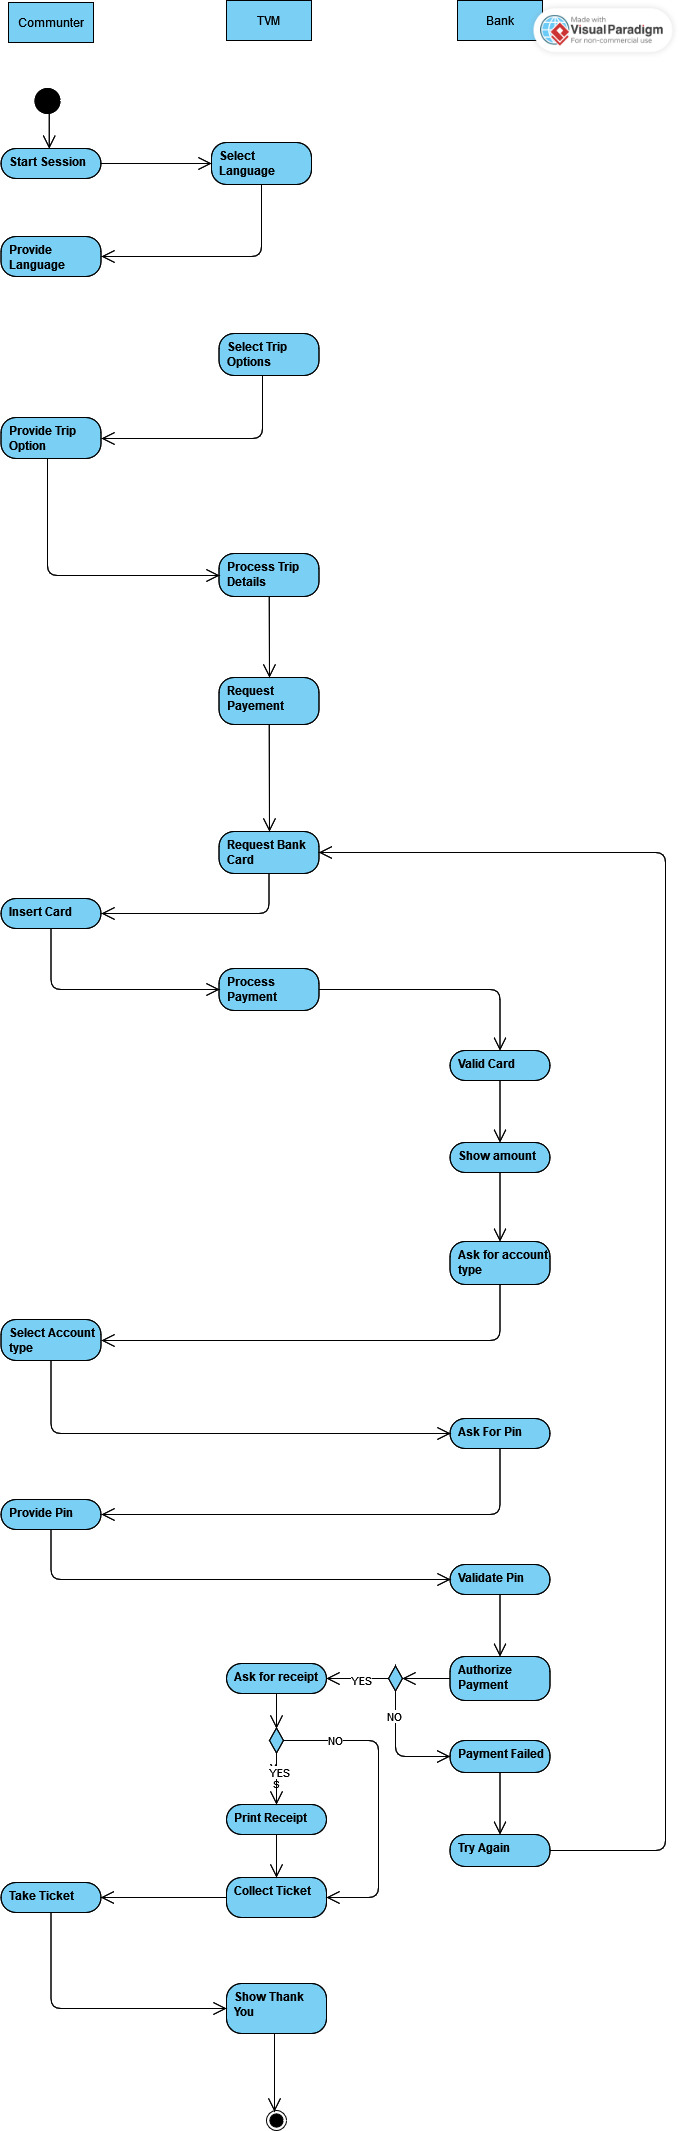
\includegraphics[width=2.085in]{Ticket.png}
        \caption{Activity Diagram (Ticket Purchase)}
    \end{center}
\end{figure}
\subsection{OPUS Recharge}
The above activity diagram shows the activity flow for a commuter to recharge the OPUS card. The computer selects the preferred language, then inserts the OPUS card in the TVM. Then, TVM shows the options that commuters can select from the list. The commuter picks the desired option. Then, TVM asks the commuter to pay for the option selected. The commuter inserts the bank card to pay through the card. The bank server validates the card, after validation the user is asked to select the account type. 
\\\
\\\The commuter selects the type and then the bank shows the amount and asks the commuter to validate the amount that will be deducted from his/her account. After confirmation, the bank asks for a pin. The commuter provides a pin and the bank validates and approves the transaction. TVM asks the commuter whether he/she needs a receipt for the transaction. Then, TVM asks the commuter to take the OPUS card out.
\begin{figure}[!p]
    \begin{center}
        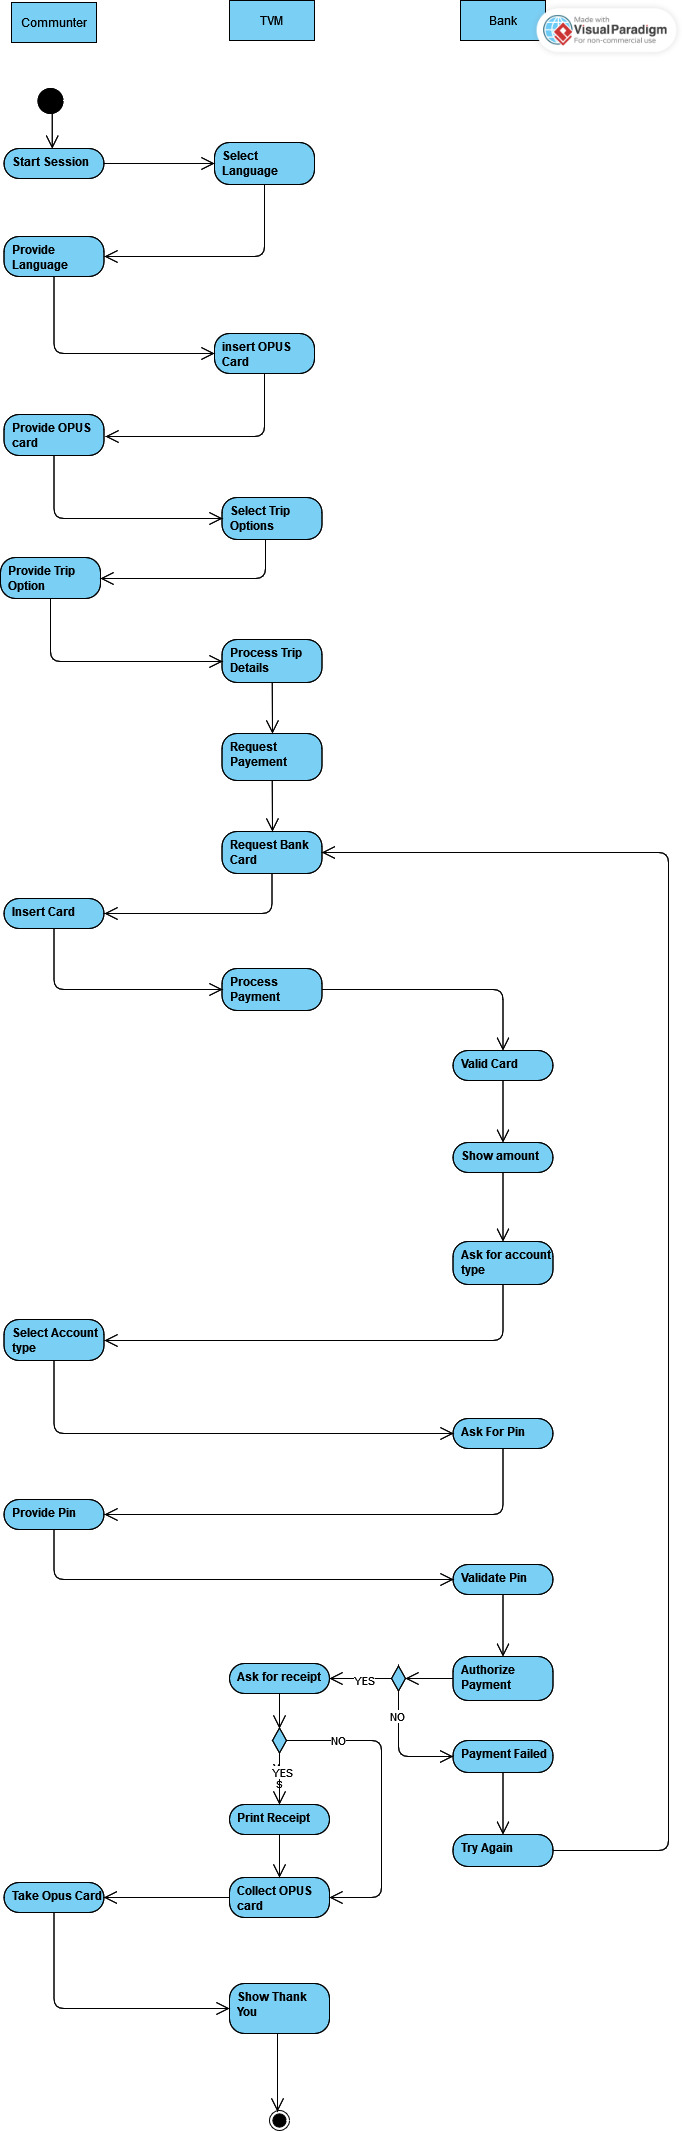
\includegraphics[width=2.4in]{Activity Diagram (OPUS).jpg}
        \caption{Activity Diagram (OPUS Recharge)}
    \end{center}
\end{figure}
\subsection{Change Ticket Fairs}
The above activity diagram shows the activities involved when an admin tries to update a fare. Admin asks TVM to show the admin page. TVM shows the admin page. From the page, admin selects the update fare option. The TVM shows two options ticket/Opus. The admin picks the option which he/she wishes to update. Then TVM shows all the options related to the selected item. Then the admin picks the trip from the list which he/she wants to update. TVM shows the current price for the trip, the admin put a new price and press update. TVM asks yes/no to proceed with the update. The admin gives yes. The TVM sends the request to the server. The server tries to update the price. Once it is updated, the server returns a success message. The admin gets a success message displayed by the TVM.
\begin{figure}[!p]
    \begin{center}
        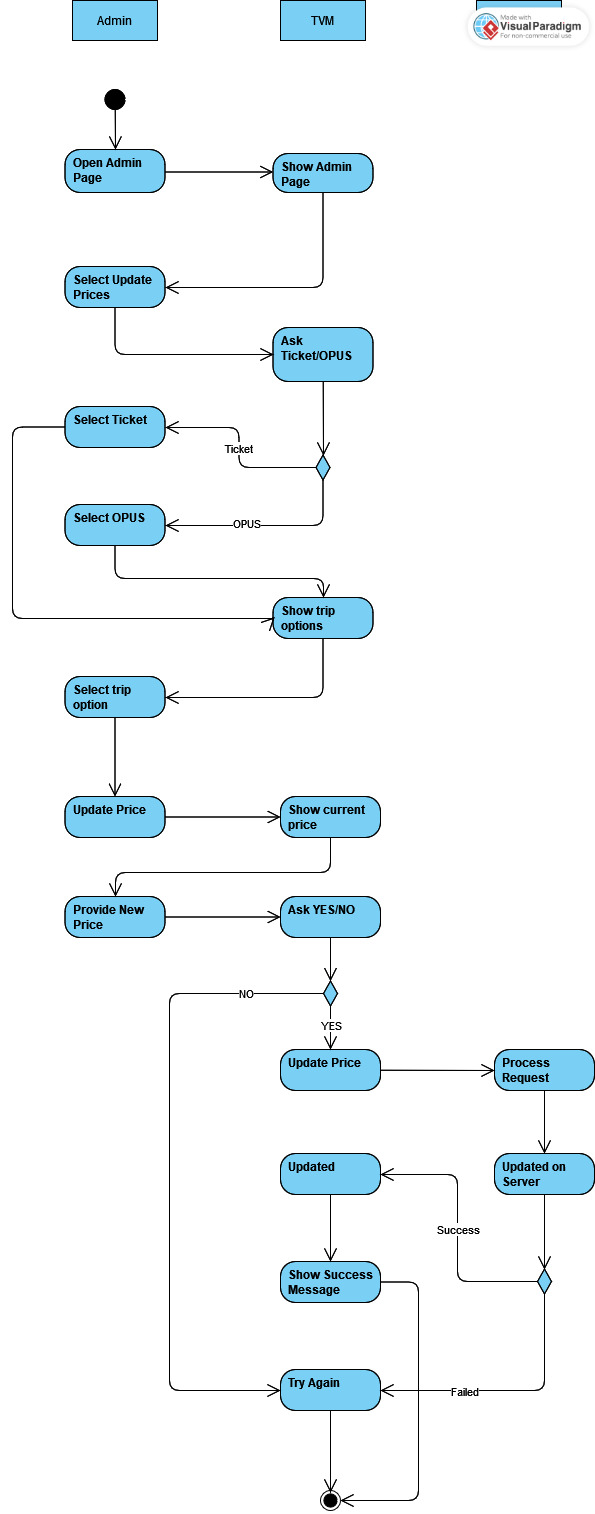
\includegraphics[width=2.9in]{Activity Diagram (Admin).jpg}
        \caption{Activity Diagram (Update Prices)}
    \end{center}
\end{figure}
\newpage
\section{Conclusion}
\textbf{\subsection{What we learned}}
At the conclusion of our project, we held a final meeting to reflect on our experiences and identify areas for improvement. We reached a unanimous consensus that we gained valuable insights into the importance of maintenance throughout the project. Additionally, we recognized that our exposure to various technologies was limited, and we had only a superficial understanding. As a result, we committed to continue our efforts and acquire a deeper understanding of these technologies.
\textbf{\subsection{What could be improved}}
The communication aspect proved to be the most challenging aspect of this project, as we, being students with different schedules, found it difficult to synchronize with each other. Despite being proactive in minimizing any impact, we acknowledged that there was still room for improvement.
\newpage
\printbibliography[heading=bibintoc,type=article,title={References}]
\end{document}